\section{Architecture}\label{sec:architecure}
Based on the concept, an architecture for a voice assistant has been developed, which can be seen in Figure \ref{fig: infrastruktur-overview}. This architecture offers more privacy and is divided into three main modules: the mobile app, the repository and the cloud. The module \glqq Speech Processing\grqq{} exists in the mobile app and in the cloud. The Mobile App implements simple speech processing such as recording or playing an audio file. Resources intensive language processing processes, such as the conversion of speech to text, are outsourced to the cloud. In the following, the three main modules are described in more detail.

\begin{figure}[h!]
	\centering
	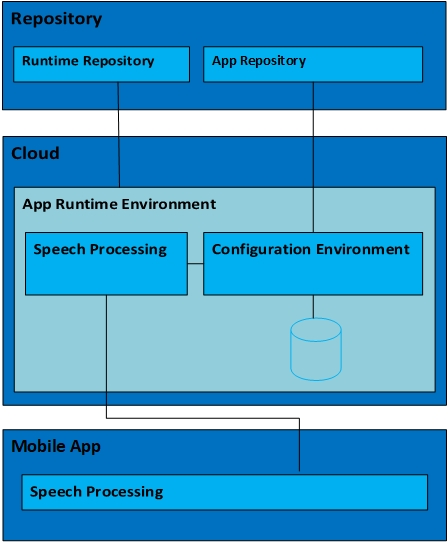
\includegraphics[width=0.8\linewidth]{Picture/Infrastruktur-Overview.jpg}
	\caption[Architecture - Overview]{Architecture - Overview}
	\label{fig:infrastruktur-overview}
\end{figure}

\subsection{Mobile App}
The mobile app is the interface to the user and as shown in Figure \ref{fig:infrastructure-app}, these three modules have:

\begin{itemize}
	\item \textsl{Speech Recording:} Record and stream a user's input to the cloud.
	\item \textsl{Speech Playback:} Play a stream created by the cloud to the user.
	\item \textsl{Hotword Detection:} The mobile app should not continuously stream the user's input to the cloud, as this could compromise the user's privacy. The app should only record and stream if the user wants it. Thus, the so-called \glqq Hotword Detection\grqq{} is used. This overhears the user consistently locally on the terminal. A hotword detection requires little resources, as it has been optimized for the detection of a single signal word. Thus, a signal word can be defined. As soon as the user says this signal word, the recording and streaming to the cloud is started.
\end{itemize}

\begin{figure}[h!]
	\centering
	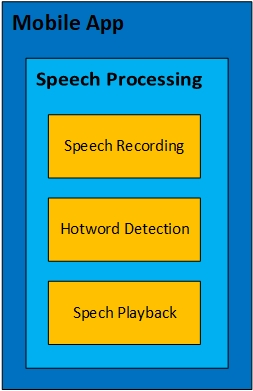
\includegraphics[width=0.3\linewidth]{Picture/Infrastruktur-App.jpg}
	\caption[Architecture - Mobile App]{Architecture - Mobile App}
	\label{fig:infrastruktur-app}
\end{figure}

\subsection{Repository}
The repository is shown in figure \ref{fig:infrastructure-repository} and is divided into two modules: the Runtime Repository and the App Repository, which are described in more detail below.

\begin{itemize}
	\item \textsl{Runtime Repository:}The Runtime Repository provides a runtime environment for the cloud. The runtime environment includes the operating system and all the packages needed by the voice assistant and is provided in various formats. A user can download a runtime environment in the format of their choice and install it on their private cloud. The installation should require as little configuration effort as possible, because even users without an IT background should be able to install these environments. 
	\item \textsl{App Repository:} The app repository provides all the apps available for the voice assistant. If a user wants to use an app, he has to install it in his runtime environment. Developers can deploy apps to users in the App Repository. However, they must provide accurate information about the use of the data of a user. Furthermore, it is checked before the publication of an app, whether the data protection information is correct and whether it needs the collected data at all for the improvement of user-friendliness. Thus, data saving for an app can be ensured.
\end{itemize}


\begin{figure}[h!]
	\centering
	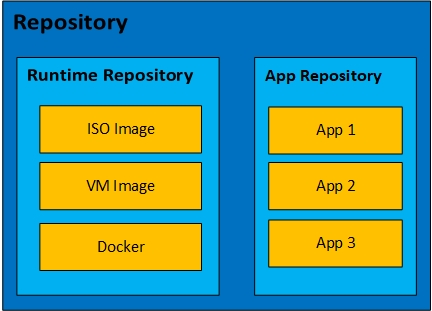
\includegraphics[width=0.6\linewidth]{Picture/Infrastruktur-Repository.jpg}
	\caption[Architecture - Mobile App]{Architecture - Repository}
	\label{fig:infrastruktur-repository}
\end{figure}

\subsection{Runtime Environment}
The runtime environment is the hearth of the voice assistant and is shown in Figure \ref{fig:infrastructure-cloud}. It contains a large amount of functions.

\begin{figure}[h!]
	\centering
	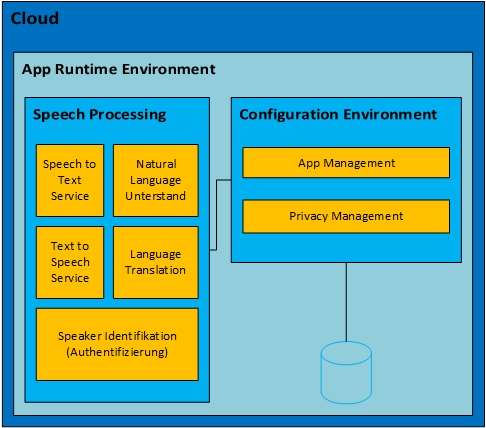
\includegraphics[width=0.9\linewidth]{Picture/Infrastruktur-Cloud.jpg}
	\caption[Architecture - Cloud]{Architecture - Cloud}
	\label{fig:infrastruktur-cloud}
\end{figure}

\begin{itemize}
	\item \textsl{Speech Processing:} The Speech Processing module contains computationally intensive voice processing functions. The following sub-areas of speech processing are required for the language assistant:
	\begin{itemize}
		\item \textsl{\ac{stt}:} \ac{stt} is the conversion of a speech signal to text.
		\item \textsl{\ac{tts}:} \ac{tts} is the conversion of a text to a speech signal.
		\item \textsl{\ac{nlu}:} \ac{nlu} is the understanding of the natural language. This is necessary to understand the input of a user. For example, it can be recognized whether a word in a sentence is a noun or verb.
		\item \textsl{Language Translation:} This involves the translation of a text into another language. This allows a user to communicate with other users who speak another language without their speaking the language. An App for the Language Assistant may not be available in the language of the user, but the contents of the app at runtime may be translated into the language of the user. This minimizes the development effort for the developers of apps while allowing a large audience of users to speak a variety of languages.
		\item \textsl{Speaker Identifikation:} The speaker identification can serve as the authentication method of the voice assistant. By the language information in a speech signal of a user this can be identified. Thus it can be checked whether a user has the right to use this language assistant.
	\end{itemize}
	\item \textsl{Configuration Environment:} The configuration environment allows you to configure the Apps and Privacy settings for the language assistant.
	\begin{itemize}
		\item App Management: This module manages the apps installed by the user. It can install new apps from the App Repository or uninstall existing apps.
		\item Privacy Management: This module manages the context of the user and allows him to set the access of apps to this context. It can be determined which information of the user is accessible from an app. Furthermore, fictive contexts can be created so that the user can use an app without abandoning his actual context. Through this module, user-controlled privacy can be achieved. 
	\end{itemize}	
\end{itemize}





